\section{Evaluation}
\label{s:eval}

\begin{figure*}
\centering
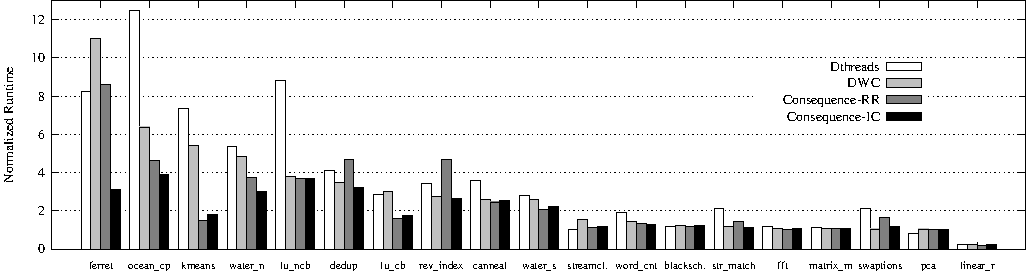
\includegraphics[width=7.0in]{figures/overall_runtimes.pdf}
\caption{\lib{}, DThreads and DWC runtime normalized to pthreads runtime. Main result shown as \lib{}-IC. \lib{}-IC achieves an average of 2.8$\times$ and 2.2$\times$ improvement over DThreads and DWC (respectively) on the five most challenging benchmark programs.}
\label{f:performance}
\end{figure*}

\begin{figure*}
\centering
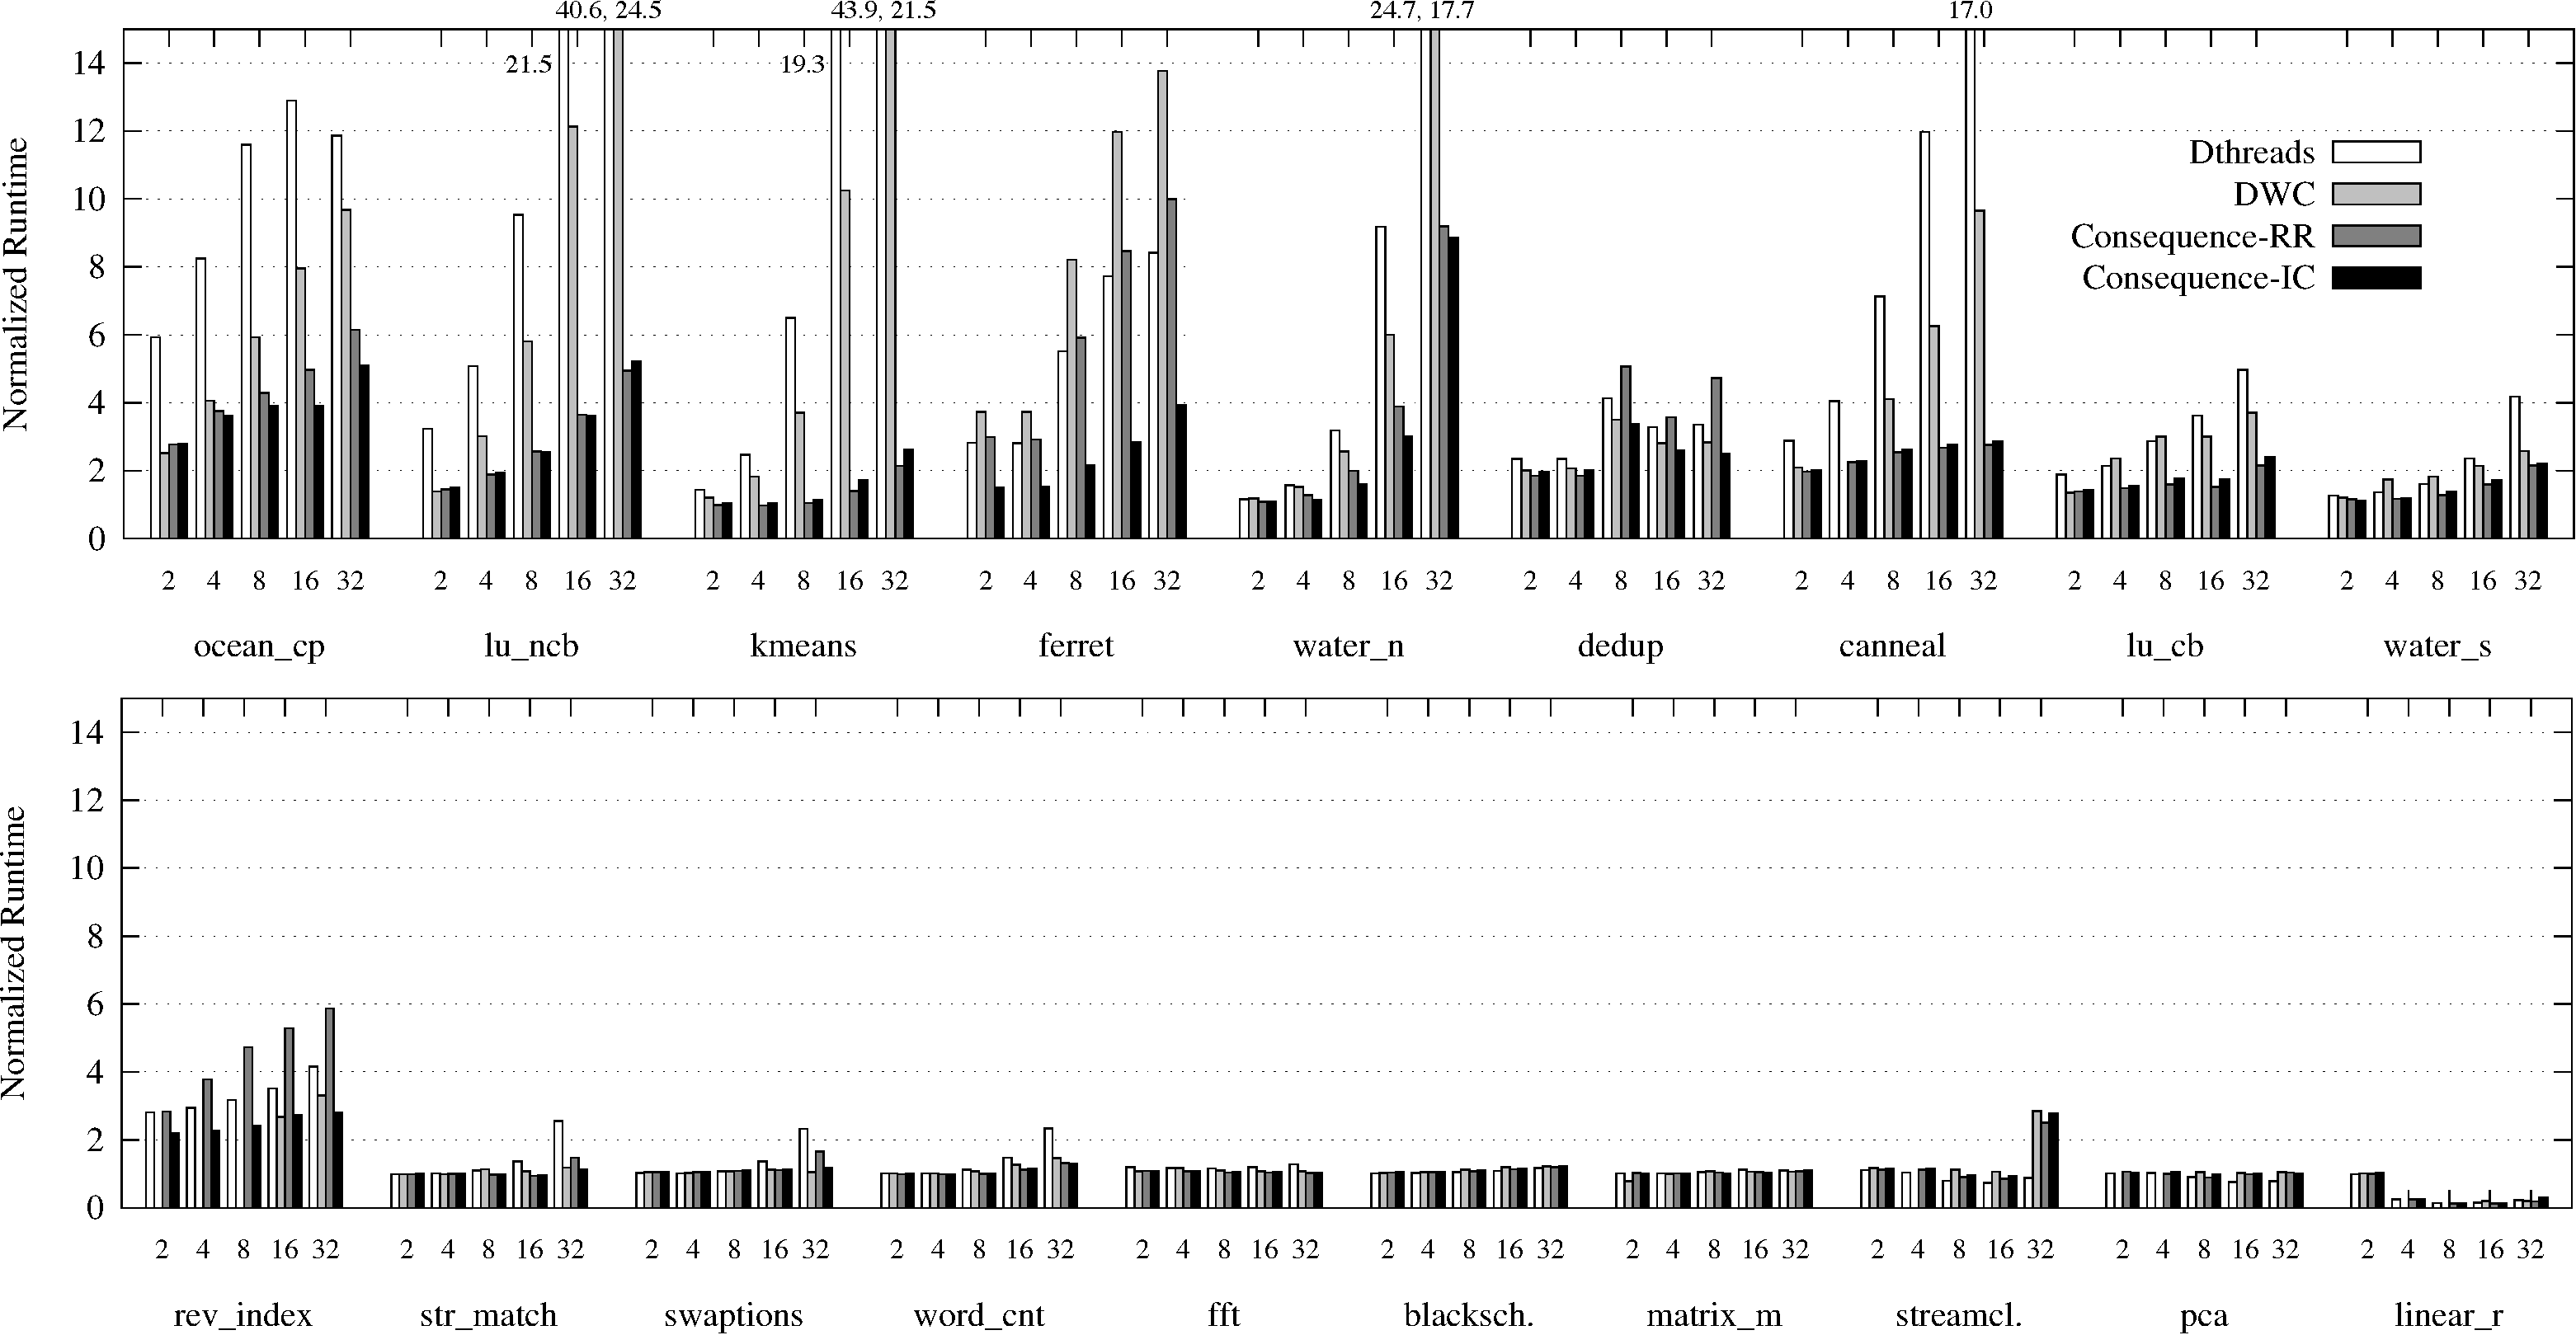
\includegraphics[width=7.0in]{figures/scalability_results.pdf}

\caption{Performance when varying the number of threads for \lib{}, DThreads and DWC.}
\label{f:scalability}
\end{figure*}

\begin{figure*}
\centering
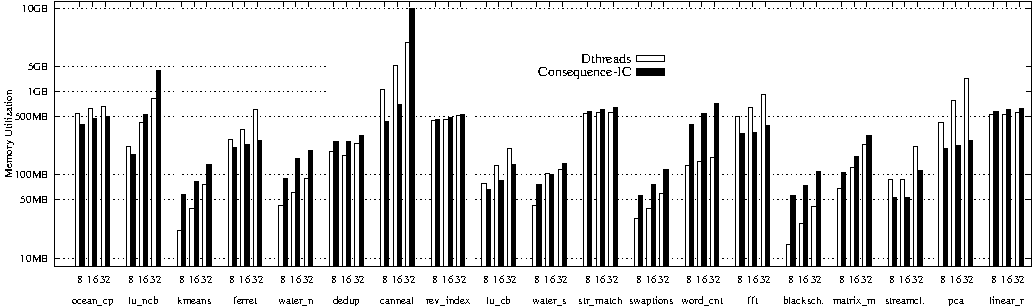
\includegraphics[width=7.0in]{figures/memory_utilization.pdf}
\caption{Peak memory usage for \lib{} and DThreads.}
\label{f:memory}
\end{figure*}

Below, we study the performance of \lib{} in broad strokes, followed by several detail studies. Our results were produced on a computer with four 2.00GHz Intel Xeon E7-4820 8-core processors and 256GB of main memory, running Linux 2.6.37 with the \conversion{} and \lib{} kernel patches. For these experiments, Hyper-threading was turned off, and the frequency scaling governor was set to \emph{performance}. Experiments were run 10 times per thread count, and mean deviation was within 20\% for all benchmarks other than {\it linear\_regression}, where the execution times can be below 500ms.

Figure \ref{f:performance} illustrates our main result: the runtime of two different variations of \lib{}, as well as DThreads \cite{liu_dthreads:_2011} and DThreads with \conversion{} (DWC) \cite{merrifield_conversion:_2013}. \footnote{Unfortunately a comparison with the relaxed consistency system RFDet \cite{kai_lu_efficient_2014} was not possible as the current implementation is provided without deterministic synchronization.} DThreads and DWC both use round-robin ordering, commits at synchronization operations and virtual memory-based isolation through either {\tt mprotect()} (DThreads) or specialized kernel support (DWC). For each library we present results from 19 benchmarks\footnote{Other benchmark programs from Parsec, Phoenix and SPLASH-2 are problematic for deterministic execution. This is mainly caused by the use of ad-hoc synchronization techniques. See \cite{liu_dthreads:_2011} for details.} from the Phoenix, Parsec and SPLASH-2 benchmark suites, normalized to pthreads runtime. 

To produce this plot, we measured the performance of each library (as well as pthreads) using 2--32 threads, and retained the corresponding best result. The plot shows the best library runtime, divided by the best pthreads runtime, for each benchmark. 

Here, \lib{}-RR uses round-robin ordering based on synchronization operations (similar to that used in DThreads and DWC), while \lib{}-IC uses GMIC ordering (see \S\ref{s:dlc}). We see a maximum slow-down vs. pthreads of 3.9$\times$ using \lib{} with the deterministic GMIC ordering (compared to 12.5$\times$ with DThreads and 11.0$\times$ with DWC). The maximum slow-down is arguably the number to watch, as many of the benchmarks are ``embarrassingly parallel'' to start with and offer little or no insight into the performance of these libraries. While DThreads and/or DWC do outperform \lib{}-IC on some benchmarks, this difference is within the mean variation for all but two programs: {\it linear\_regression} and {\it pca}. Further, all cases where a \lib{} variant is not the top performer occur for programs where the max slow-down is less than 2.0$\times$ pthreads across all libraries. 

An interesting result occurs on the {\it reverse\_index} and {\it dedup} benchmarks, where \lib{} is negatively impacted by its more sophisticated and flexible locking algorithm. Both DThreads and DWC treat each lock as a single global lock, which works well for programs where there is only a single lock and critical sections are short. This causes \lib{}-RR performance to suffer, yet \lib{}-IC still manages to provide the best performance by generating a better deterministic ordering.

Figures \ref{f:scalability}--\ref{f:memory} analyze the scalability of \lib{} with respect to thread count, in terms of runtime and memory usage. These reveal a severe DThreads and DWC scalability problem for six benchmarks: {\it  ocean\_cp, lu\_ncb, ferret, kmeans, water\_nsquared} and {\it canneal}. \lib{} also exhibits scaling difficulties, albeit much less severe. 

On the {\it water\_nsquared} benchmark with 32 threads, \lib{} experiences a drastic and unexpected performance hit. This occurs because each thread performs many fine-grained lock acquisitions with short critical sections, which become coarsened with \lib{}. Because a thread holds on to the token throughout the entire coarsened chunk, other threads may be blocked, leading to the scalability issue seen here.

In terms of memory usage (see Figure \ref{f:memory}), DThreads and \lib{} appear evenly matched. Two notable exceptions are {\it canneal} and {\it lu\_ncb} at high thread counts. This is caused by a high volume of page allocation/freeing such that the single-threaded \conversion{} garbage collector cannot keep up. A multi-threaded collector would solve this issue.

\subsection{Sources of Performance Improvement}

As described in \S\ref{s:optimizations}, \lib{} includes a number of performance optimizations, aimed at reducing the cost of common concurrency patterns. To better understand how these various parts contribute to the performance of \lib{}, we evaluate \lib{}-IC with and without each of these optimizations.

\begin{figure}
\centering
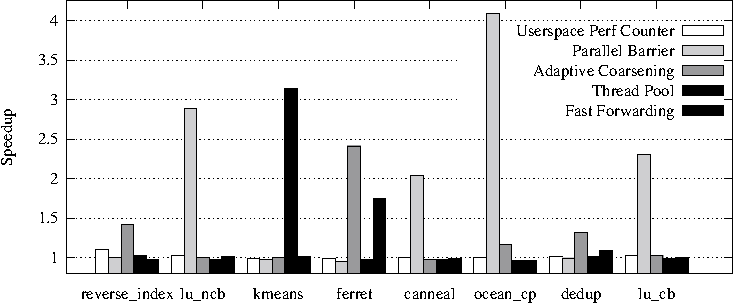
\includegraphics[width=3.3in]{figures/optimizations.pdf}
\caption{Speedup (higher is better) of various optimizations on a select group of benchmarks.}
\label{f:optimizations}
\end{figure}

Figure \ref{f:optimizations} shows the performance improvement (higher is better) contributed by each of five major optimizations, on eight of the most difficult benchmarks. While all optimizations demonstrate some amount of improvement, we find that user space performance counter readings contribute very little to the overall performance. For {\it ferret}, being one of the hardest of the benchmark programs to perform well on, both the adaptive coarsening and fast forward optimizations provide major speed improvements. For {\it ocean\_cp, lu\_ncb, canneal} and {\it lu\_cb} the parallel barrier provides the main source of our speedup. Note that these numbers represent the performance difference in \lib{} with and without each optimization, not a performance improvement with respect to pthreads or DThreads. 


\begin{figure}
\centering
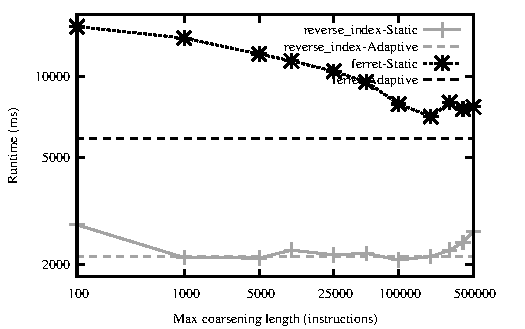
\includegraphics[width=3.1in]{figures/adaptive.pdf}
\caption{Comparison of Adaptive and Static Coarsening for {\it reverse\_index} and {\it ferret}. }
\label{f:adaptive}
\end{figure}


Adaptive Coarsening stands out as one of the most successful optimizations, which merits additional study. Figure \ref{f:adaptive}, shows the effect of coarsening level (x-axis) on the runtime (y-axis, lower is better) of the {\it reverse\_index} and {\it ferret} benchmarks. It is clear that the coarsening level has a significant effect of runtime performance, even when set statically. With adaptive coarsening, each thread selects its own coarsening level, allowing adaptive coarsening to outperform even the best statically chosen coarsening level. 

\subsection{What is Holding \Lib{} Back?}
\begin{figure*}
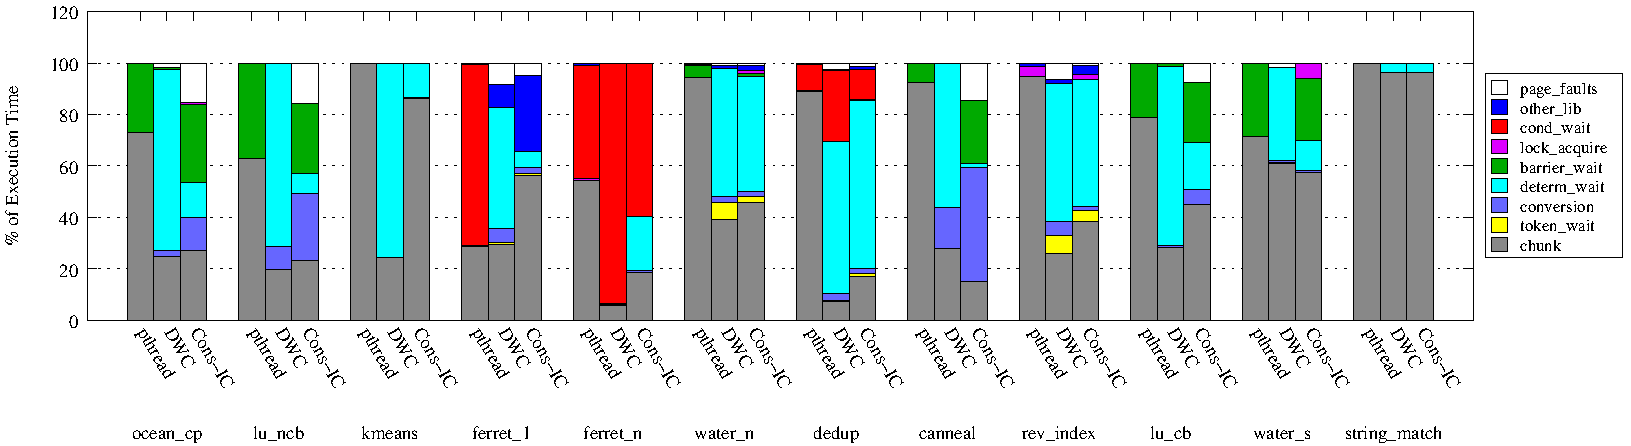
\includegraphics[width=7.0in]{figures/fine_grained_analysis.pdf}
\caption{Breakdown of the time spent in each benchmark with pthreads, DWC and \lib{}-IC using 8 threads.}
\label{f:fine-grained}
\end{figure*}

Figure \ref{f:fine-grained} provides a breakdown of where \lib{} spends time for a selection of benchmarks. The benchmarks can be divided between ``embarrassingly parallel'' ({\it string\_match}), barrier-heavy ({\it ocean\_cp, lu\_cb, lu\_ncb, canneal, water\_nsquared and water\_spatial}) and those that experience other determinism-related overhead ({\it kmeans, ferret, dedup and reverse\_index}). For {\it ferret}, the first thread spawned is presented on its own ({\it ferret\_1}) because it exhibits a radically different synchronization pattern than the rest ({\it ferret\_n}).

For the barrier-heavy programs (e.g. canneal), DWC typically has a much higher execution time (see Figure \ref{f:scalability}) and a large percentage of that time is spent waiting on others. This is because the DWC barrier commits are done serially and the amount of memory that must be committed is typically high. In \lib{}-IC, much of the commit work is done in parallel so the wait time (shown as barrier\_wait\footnote{We separate barrier\_wait and determ\_wait time for \lib{} because the time spent waiting at the barrier is not impacted by deterministic ordering.}) is greatly reduced. With less wait time, the remaining overhead is spread between copy-on-write page faults and commit operations in \conversion{}. For {\it canneal} and {\it lu\_ncb} the time spent in \conversion{} is higher because threads tend to write to the same page in isolation, leading to a larger number of byte-granularity merges.

The {\it ferret} program provides an interesting challenge for deterministic execution. The first phase of the pipeline (shown as {\it ferret\_1}) performs a high volume of lock acquisitions with short chunk sizes, while the rest of the threads oscillate between executing longer chunks and waiting at conditional variables. For good deterministic performance, it is important to (1) provide an ordering that allows the first thread to perform synchronization unimpeded, and (2) reduce the cost of each synchronization operation. \lib{}-IC provides (1) through GMIC ordering and (2) through adaptive coarsening. This results in more time spent executing chunks and less time spent waiting or performing page faults.\footnote{Coarsening can reduce the total number of page faults if two chunks in a coarsened chunk write to the same page.}. \lib{}-IC still experiences a large amount of general library overhead on {\it ferret\_1} which is mainly caused by reading the performance counters and other work done between chunks.

\subsection{Memory Propagation for Relaxed Models}

For some benchmark programs like {\it canneal} and {\it lu\_ncb}, the amount of memory that must be propagated between threads can degrade \lib{} performance. Therefore, it is worth investigating whether relaxed memory models can perhaps alleviate this burden on deterministic execution.

An LRC-based memory model can reduce total memory propagation by allowing commits to be "point to point." More specifically, memory is propagated between threads using the \emph{happens-before} relation. An operation $a$ is said to have happened before $b$ if (1) $a$ occurs before $b$ within the same thread of execution, or (2) $a$ and $b$ are release and acquire operations on the same synchronization variable. 

To evaluate the reduction in memory propagation that a relaxed memory model can offer, we modified \lib{} to track the happens-before relation. This was achieved by adding a vector clock to each thread, synchronization variable and committed page. For each acquire operation (lock, conditional wait, thread creation/join and barrier wait)\cite{kai_lu_efficient_2014}, we compute which pages would need to be propagated along happens before edges.

Figure \ref{f:tsovslrc} compares the total number of pages propagated under TSO (\lib{}) and the expected number for an LRC-based system across 12 benchmarks that perform at least 10K page updates. While the LRC system can reduce total memory propagation, the reduction is just 21\% when averaged across all benchmarks considered. For some benchmarks like {\it canneal}, the use of barriers limits the gains from using a relaxed consistency model.

